\chapter{Senzory a akční plány}


V této kapitole se již přesouváme od hry samotné ke způsobu, jak na daný stav hry nahlížet chytřeji a také, jak na něj lépe reagovat. 
Na nejnižší úrovni herní prostředí vrací v každém kroku stav hry, který obsahuje seznamy všech vesmírných objektů a úkolem agentů je na něj reagovat vybráním elementární akce.
V této kapitole se zaměříme na abstrakce, které z obsáhlých a detailních informací nízké úrovně získají menší objemy zajímavějších informací vyšší úrovně. 
Podobně jako abstrakce nad herním stavem budeme chtít vytvořit i abstrakce nad akcemi agentů, jejich cílem bude namísto volby elementárních akcí nízké úrovně volit akce vyšší úrovně.
A právě tyto abstrakce realizujeme pomocí senzorů a akčních plánů.
\section{Senzor}

Senzorem nazveme metodu, která z detailního stavu reprezentovaného seznamem vesmírných objektů extrahuje informaci vyšší úrovně, která není ve stavu explicitně zadána.
Informace získané z těchto senzorů, respektive senzorických metod, můžeme využít v rozhodovacím problému vybírání akcí.
Většina senzorických metod v rámci svého výpočtu využívá simulování hry. 
Simulace na základě současného rozpoložení všech vesmírných objektů ve stavu pokračuje v pohybu všech objektů tak, jak by hra probíhala obvyklým způsobem. 
V simulaci žádný z hráčů neprovádí žádné akce, kromě těch, na jejichž dopad se v dané simulaci dotazujeme.
Ze simulace můžeme zjistit jaké konkrétní události nastanou v nejbližších krocích hry.
Všechny simulace pokračují ve hrání hry jen omezený počet kroků. Tento počet kroků je roven konstantě \emph{\uppercase{Impact\_radius}}. Pro tuto hodnotu se mi ukázal být vhodný počet 25.
Je to hodnota dostatečně vysoká na to, aby senzorické metody včas zaznamenaly potřebné informace a zároveň je dostatečně nízká, aby nebyly výpočetně příliš náročné.
Kromě senzorů, které využívají pro výpočet simulování hry, existují i senzory, jejichž výpočet probíhá nad současným stavem staticky bez nutnosti simulace.



\subsection{Příklady senzorů}
\begin{itemize}
    \item První sražený neutrální asteroid - Zde se simuluje pohyb vesmírné lodi, střel a neutrálních asteroidů. 
    V případě srážky vesmírné lodi s neutrálním asteroidem vrací tento senzor daný neutrální asteroid a počet kroků, po kterém ke srážce došlo.
    Do simulace se zahrnují i vlastní střely hráče. V případě sestřelení asteroidu střelou, jsou střela i asteroid z následné simulace odstraněny.    
    \item První sražený nepřátelský asteroid - Jde o téměř identický senzor. Jediným rozdílem je zde, že se senzor nesoustředí na asteroidy neutrální, ale nepřátelské.
    \item Asteroid zasáhne nepřátelskou loď - V této simulaci se pohybujou pouze konkrétním asteroidem a nepřátelskou lodí.
    Senzor vrací informaci zda, a případně v kolika krocích simulace se asteroid střetl s nepřátelskou lodí.
    V simulaci nepřátelská loď neprovádí žádné reakce.
    \item Střela zasáhne konkrétní asteroid - Jde o simulaci podobnou předchozí. Simuluje se pohyb konkrétního asteroidu a konkrétní střely.
    \item Střela zasáhne libovolný asteroid - Simuluje se pohyb konkrétní střely a všech neutrálních a nepřátelských asteroidů.
        Tato senzorická metoda vrací zda střela zasáhla sestřelila asteroid, daný asteroid a počet kroků, po kterém k sestřelení došlo.
    \item Vzdálenost dvou bodů - Vrátí vzdálenost dvou bodů v Euklidovské metrice.
    \item Přepočítání nejbližší polohy asteroidu od vesmírné lodi - 
        Vesmírný prostor je v jistém pohledu cyklický, proto se pro získání nejkratší vzdálenosti asteroidu od vesmírné lodi nemůžeme spolehnout na vzdálenost jejich současných poloh, ale musíme vzít v úvahu všechny čtyři polohy asteroidu.
        Ty získáme postupným posunutím asteroidu o šířku a délku prostoru.
        Jinými slovy vzdalenost vesmírné lodi od asteroidu posunutého přes hranici prostoru může být kratší než přímá vzdálenot k původní polohy asteroidu.
    \item \emph{N} nejblizších asteroidů od vesmírné lodi - Tento senzor spočítá nejkratší vzdálenosti vesmírné lodi od všech asteroidů ve hře a vrátí relativní polohu \emph{N} nejbližších z nich.
    
\end{itemize}


\begin{figure}[hp]

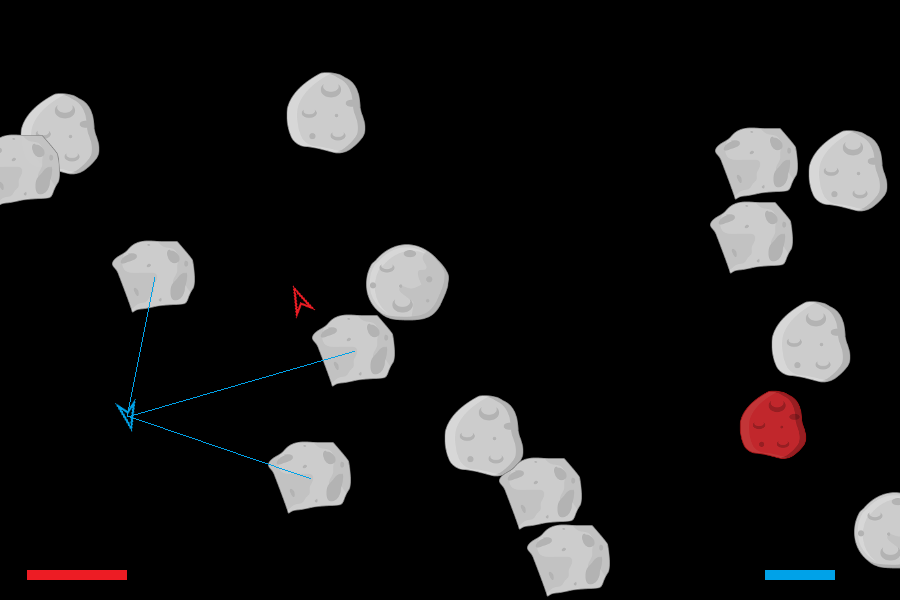
\includegraphics[width=145mm, height=100mm]{./Obrazky/N_nearest_asteroids.png}
\caption{Ukázka senzoru "\emph{N} nejbližších asteroidů od vesmírné lodi" pro \emph{N}=3}
\label{obr02:}
\end{figure}


\section{Akční plán}
Druhou zmíněnou abstrakcí jsou akční plány, jejich cílem je podobně jako u senzoru pracovat namísto akcí nízké úrovně s akcemi vyšší úrovně. V případě akcí toto znamená namísto volby jednotlivých elementárních akcí volit akční plány, který mají komplexnější cíl.
Akční plán reprezentuje posloupnost elementárních akcí, které má agent vykonávat v následujících krocích hry.
Cíl akčního plánu se liší podle toho, o jaký druh se jedná.
\par
Podobně jako u senzorických metod i zde hledání většiny akčních plánů probíhá simulací hry.

\subsection{Jednotlivé plány}
\begin{itemize}
    \item Útočný plán - 
        Tento akční plán hledá posloupnost rotací následovaných střelou tak, aby byl sestřelen asteroid, který poté zasáhne nepřátelskou loď.        
        Simulace inkrementálně prochází všechny možné otočení a následné střely. Vesmírná loď se v rámci simulace otočí, vystřelí se střela a následně se sleduje, zda tato střela zasáhne libovolný velký nebo střední asteroid.
        Nad tímto asteroidem se následně zkouší, zda-li asteroidy vzniklé rozstřelením zasáhnou nepřátelskou loď. Rozstřelení asteroidu se zkouší pro oba typy střel.
        \par
        V případě nesestřelení žádného asteoridu, nebo minutí nepřátelské lodi rozstřeleným asteroidem, se v simulaci vesmírná loď pokusí provést další rotaci a celý pokus o střelbu opakovat.
        Pokud v simulaci nastalo úspěšné sestřelení, tak se vrací útočný akční plán, který obsahuje přílušný počet rotací následovaný střelou.
    
    \item Obranný plán - Pro hledání obraného plánu je nejprve potřeba vědět, před kterým asteroidem je potřeba vesmírnou loď bránit. 
        Zde využijeme připravené senzory. Posloupnost obraného plánu obsahuje dvě části. V První části se vesmírná loď rotuje tak, aby mířila na asteroid, před kterým je potřeba se bránit.
        A v druhé části probíhá samotná střelba, ta spočívá v jediné elementární akci střelby. Pro vyhodnocení, zda vystřelením střely sestřelíme konkrétní asteroid, využijeme připravené senzorické metody.
        \par
        Nalezení potřebné rotace pro nasměrování vesmírné lodi k nebezpečnému asteroidu probíhá statickým výpočtem bez použití simulace.
        Nejprve zjistíme přesnou polohu, kde k potenciální srážce dojde. V případě, že vesmírná loď, anebo asteroid stojí staticky na místě, tak ke srážce dojde na současné poloze vesmírné lodi.
        V případě pohybu obou objektů se poloha střetu nachází na průniku jejich trajektorií. Tuto polohu střetu musíme vzít v úvahu při nasměrovávání vesmírné rakety k asteroidu.        
        Pokud by se vesmírná loď otočila pouze vzhledem k současné poloze asteroidu, tak by vystřelením mohla letící asteroid minout.
        Proto namísto současné polohy asteroidu musí vesmírná loď mířit na cílovou polohu.
        Cílová poloha pro nás bude bod, který leží na úsečce spojující současnou polohu asteroidu a polohu střetu objektů a to ve vzdálenosti 15\% jejich vzdálenosti blíže k poloze asteroidu. 
        Tímto způsobem bude vesmírná loď mířit mírně před asteroid do jeho trajektorie. Empiricky jsem vyzkoušel, že tato vzdálenost v praxi funguje velmi dobře.
        Po vypočtení cílové polohy stačí spočítat rozdíl současného úhlu vesmírné lodi od úhlu směřujícímu k cílové poloze. A z tohoto rozdílu snadno získáme potřebný počet rotací. Ty budou tvořit výsledný obranný plán.
        
    
    \item Úhybný plán - Jedná se také o defenzivní plán, ale namísto přímého sestřelení nebezpečného asteroidu se tento akční plán snaží asteroidu vyhnout.
    Podobně jako u obranného plánu potřebujeme vědět před jakým asteroidem je potřeba se vyhnout. Tento asteroid je stejně jako v předchozím obranném plánu získaný senzorem. Po nalezení nebezpečného asteroidu simulace postupně prochází všechny možné otočení a následnou akceleraci.
    Počet potřebných akcí akcelerace probíhá také inkrementálně. Nejprve se vyzkouší provedení jedné akce akcelerace a následně se simuluje pohyb vesmírné lodi a asteroidu bez dalšího akcelerování.
    Při srážce vesmírné lodi s asteroidem se oba objekty vrátí na původní místo a vyzkouší se o jednu akci akcelerace více než v předešlém případě.
    V případě úspěšného vyhnutí bude úhybný akční plán obsahovat posloupnost akcí rotace následované posloupností správného počtu akcí akcelerace.
    
    \item Zastavovací plán - Tento plán jsem vytvořil na základě sledování chování agenta využívajícího úhybný plán. Úhybný plán vždy vrací nejkratší možný plán, který stačí na vyhnutí se srážce. Jako důsledek proto obvykle plán obsahuje minimální počet rotací, který je dostačující.
        To mělo v praxi za následek, že agent, který se řídí pouze úhybními plány používá akceleraci mnohem častěji než rotace a lítá proto obrovskou rychlostí přibližně stejným směrem napříč prostorem. Proto mě napadlo vytvořit akční plán, který vesmírnou loď uvede do klidu.
        \par
        Zastavovací plán má přímočarou myšlenku. 
        Nejdříve se vesmírná loď otočí tak, aby byla nasměrována proti směru svého pohybu a následně provede potřebný počet akcelerací, aby zpomalila až do úplného zastavení. 
        V tomto akčním plánu není potřeba provádět simulaci, výpočet potřebného počtu rotací i následných akcelerací lze spočítat statickým výpočtem.
        
        \par
        V kombinaci s úhybným plánem se agent chová v jistém smyslu klidněji.
        Namísto zběsilého letu napříč prostorem se vesmírná loď po vyhnutí asteroidu zastaví.            
        \par
        Tento akční plán jsem vytvořil na základě svého lidského instinktu, jak bych očekával od inteligentního agenta, že by se mohl chovat. Zda bude mít tento akční plán v praxi reálný přínos uvidíme v pozdější kapitole, kde budeme s akčními plány experimentovat.
        
        
\end{itemize}


\subsection{Přepočítávání akčních plánů}
Získávání akčních plánů je výpočetně náročné, proto jsem se pokusil jejich přepočítávání vhodně omezit. Akční plány nám vracejí posloupnost akcí na více kroků dopředu a proto není vždy potřeba je přepočítávat v každém kroku.
Změny mezi dvěmi po sobě jdoucími stavy hry nejsou veliké, ale mohou být občas dostatečné na to, aby se přepočítaný plán lišil od toho spočítaného v předchozím kroku.
V každém kroku hry se proto rozhoduje, zda se daný plán přepočítá, nebo se bude následovat plán původní. 
Plán se bude přepočítávat ve dvou možných případech, těmi jsou uplynutí daného počtu pasivních kroků, ve kterých jsme pouze pokračovali v již vytvořeném původním plánu, a nebo jeho dokončení.
Počet neaktivních kroků, po kterých dochází k přepočítávání plánu, se rovná konstaně \emph{\uppercase{inactive\_steps\_limit}}. 
S vyšším počtem pasivních kroků se velmi výrazně snižuje výpočetní čas potřebný k odehrání hry, ale počet kroků, který hra trvala, se sníží jen minimálně (viz obr03).
Je zde vidět, že kvalita hráčů se mírně snižuje, ale v porovnání kolik se ušetří výpočetního času, je tato ztráta kvality zanedbatelná.
V příštích kapitolách se nám bude pro učení agentů hodit odehrát velké množství her, proto si dovolíme nastavit vyšší počet pasivních kroků.


\begin{figure}[hp]

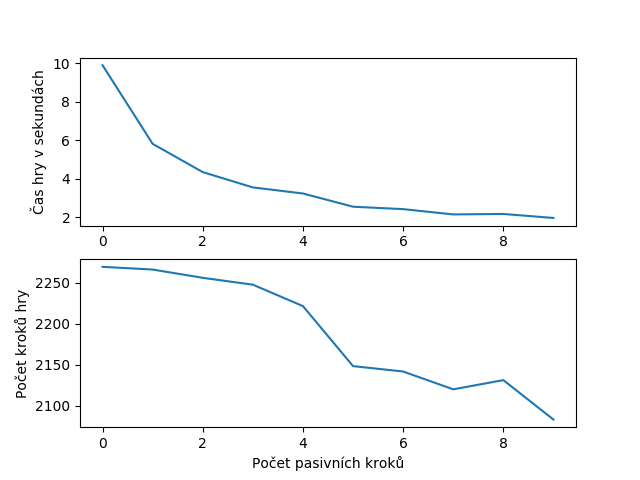
\includegraphics[width=145mm, height=120mm]{./Obrazky/Inactive_steps_comparison2.png}
\caption{Srovnání počtu neaktivních kroků k průměrné délce hry. Čísla byla získána průměrováním 40 her, kde proti sobě hráli agenti využívající pouze obranných plánů.}
\label{obr03:}
\end{figure}

\subsection{Použití akčních plánů}
Metody, které vypočítávají akční plán vracejí kromě plánů samotných i jejich délku. 
V případě nenalezení akčního plánsu se místo jeho délky vrací konstanta \emph{\uppercase{not\_found\_steps\_count}} vysoké hodnoty, ta reprezentuje, že akční plán neexistuje.
Díky tomu lze tyto metody použí také jako senzorické metody. 


